\documentclass{article}
    \usepackage{caption}
    \usepackage{subcaption}
    \usepackage{mathtools}
    \usepackage{algorithm2e}
    
    \usepackage{enumerate}% section item
    \usepackage{amssymb}  % \varnothing
    \usepackage{booktabs} % insert table
    \usepackage{multirow} % table combine
    \usepackage{listings} % insert code
    \usepackage{appendix} % 
    \usepackage{amsmath}  % for mathfont
    \usepackage{unicode-math} % for mathfont
    \usepackage{fontspec} % set font
    \setmainfont{Times} % main font
    \newfontfamily\monaco{Monaco} % code font
    \usepackage{pythonhighlight} % python
   % \usepackage{hyperref}




    \usepackage[colorlinks=true]{hyperref} % the option is there to remove the square around links which is what I don't like.
    
    \usepackage{perpage} 
    \MakePerPage{footnote} % Reset the footnote counter perpage. may require to run latex twice.
    
    \usepackage[margin=2cm]{geometry} % This is here to fit more text into the page.
    
 %   \setcounter{secnumdepth}{1}  % This removes the numbering from the subsections.
                            % If you want the numbering of the subsection level just remove this line
    
    \title{\textsc{COMP7506 - CourseSchedule}}
    \author{	
                3035562502 - ZHANG Kai \\
                3035562100 - WANG Dezhao \\
                3035562069 - YAN Qiangyu }
    \date{}
    
    \setlength{\parindent}{0pt} % No indentation for paragraphs. Because that is just old.
    \setlength{\parskip}{\baselineskip} % Instead use vertical paragraph spacing.
    
    %\setmainfont{Helvetical} % Setting the main font here. But I like the default font alot so this is commented out.
    
    \begin{document}
    \maketitle
    
    
    \section{Background Research}

    \subsection{Category \& Function Synopsis}
    CourseSchedule is an educational Android application that aims to 
    make HKU students get their course schedule easier.
    
    In this App, students can get their course schedule
    once they logged in with right portal account, 
    and it's the main function of this App.
    With this App, users can view their course with different colors.
    Meanwhile, this App also provides the function of GPA calculator,
    add the events to calendar, add notes, check the exam time, etc.

    \subsection{Market Analysis}
    There are some similar educational App in the market, 
    have different features and functions,
    but most of them only provide the course schedule of \textbf{mainland universities}.
    
    HKU as an international university has thousands of students 
    all over the world, and they all need to view the course information
    whenever they go to school. 
    Usually, students get the course information by visiting the HKU website.
    For CS postgraduate programme students, they need to view 
    the course information via CS intranet, which is more difficult for
    the App that posted in the App store to get.
    
    Based on these fact and considering the inconvenience of 
    checking the course information of
    CS postgraduate programme students in HKU, 
    we designed this App, and we believe that
    this App will have a considerable market.
    With this App, students will be able to check their course schedule
    more easier, and their only need to log in this App only once,
    this is one of its conveniences.

    Besides, this App provides the function of checking the exam timetable,
    which transform the big exam timetable 
    which shows all the exam that faculty holds into 
    the specific exam timetable of users themselves.
    And along with the timetable, it also comments with the notes
    given by the office, such as "bring the calculator", 
    "bring A4 paper sheet".
    Thus users do not need to check the informs one by one, 
    this is another of its conveniences.

    With these main features, students of CS postgraduate programme
    may have a motivation to download this App, and with the download,
    they will find this App have more useful functions like 
    GPA calculator, calendar adding and making notes.
    These functions will help users to schedule their time more easier
    and have benefits on their study, which are attractive for students.

    Even constrain this App's target users to 
    the student of CS postgraduate programme, 
    it will have a "big" market based on the consideration of
    the time cost in its developing.
    This App will have a considerable market because of 
    its own useful functions and the fact 
    that the market did not provides any similar Apps 
    that can applied out of mainland.

    Once we got more supports by other departments, 
    this App may be popular in the whole school of HKU.





    \subsection{Similar Apps}
    \subsubsection{QSC}
    \begin{center}
        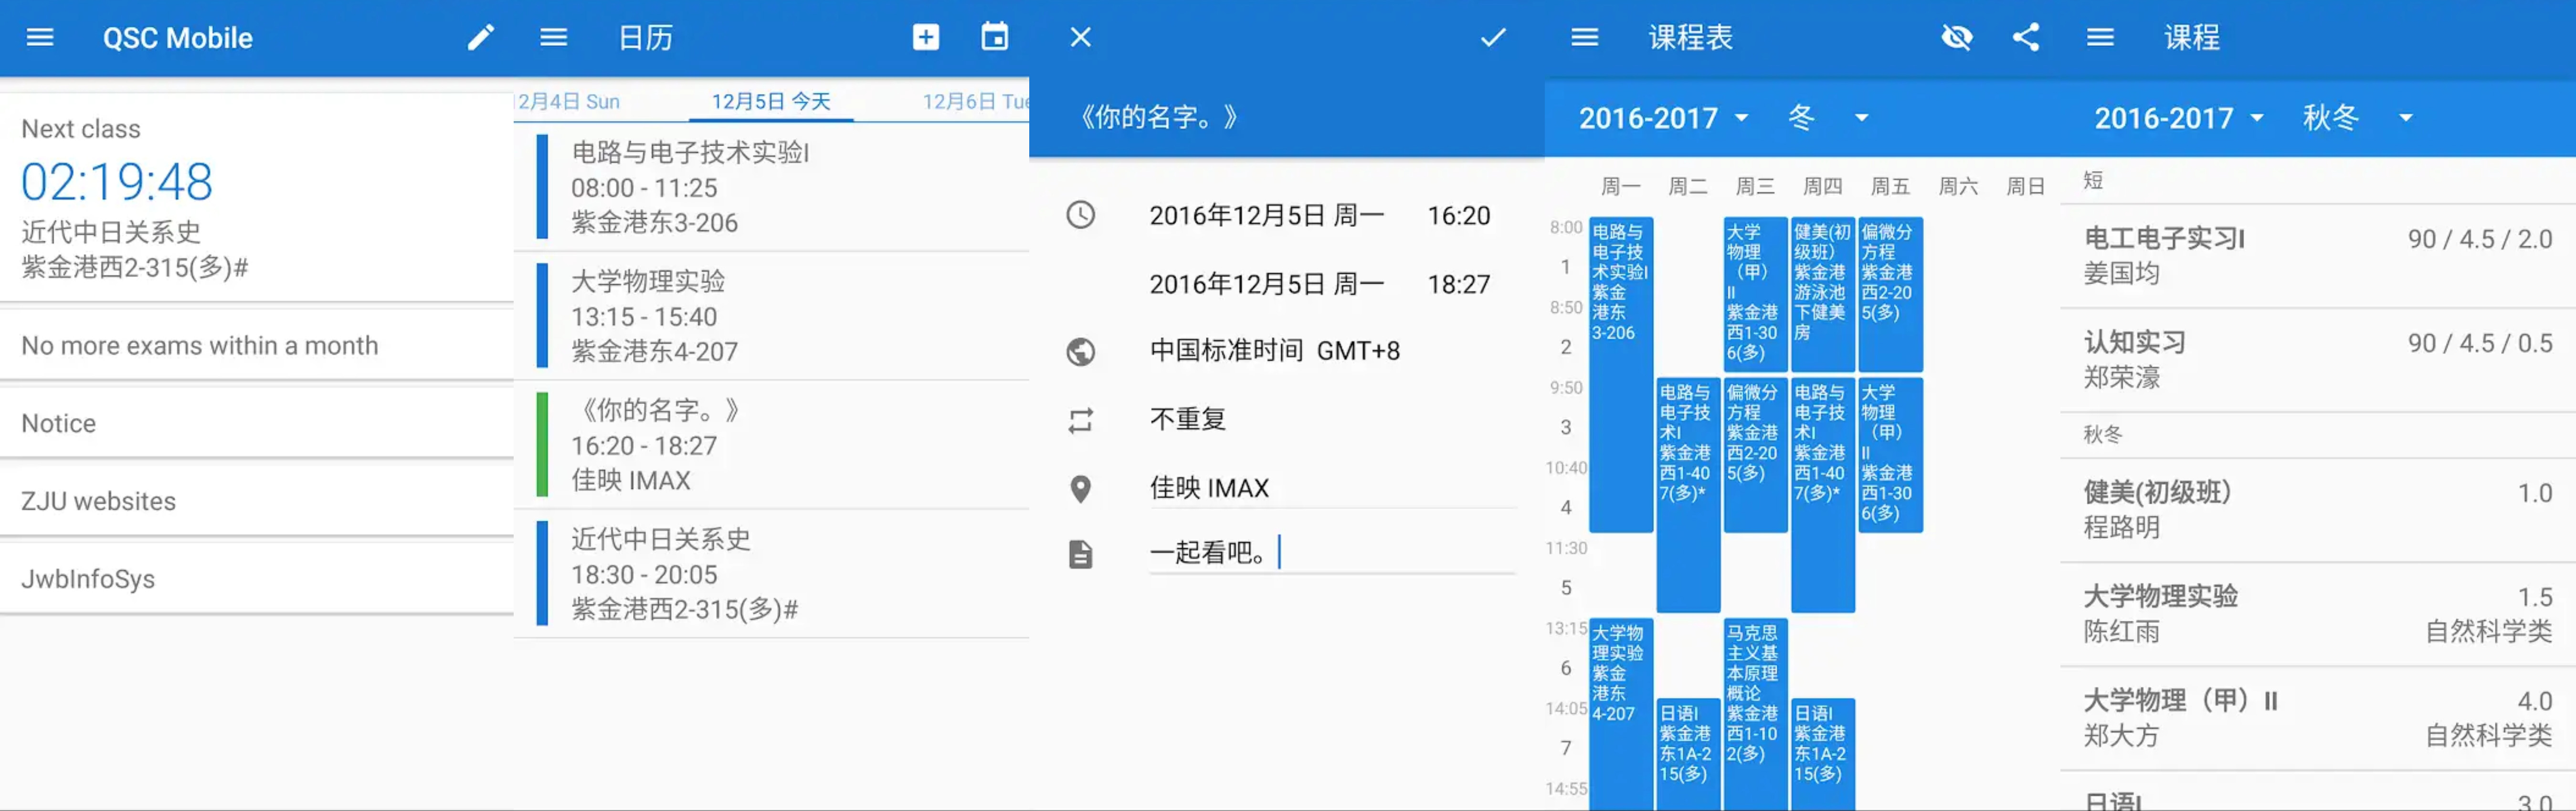
\includegraphics[width=6.9in]{QSC}
    \end{center}
    \begin{enumerate}[i)]

    \item Main Features

    - Show course schedule in days and weeks, with exam countdown.

    - Users can add the calendar to this App.

    - Review users' GPA.

    - Check the useful website.

    \item Short-Comings / Possible Improvements
    
    - Only provide the service for Zhejiang University.
    
    - All the course looks similar.

    - Other web information are just copy to the App.

    \end{enumerate}
    

    \subsubsection{CourseGrid}
    \begin{center}
        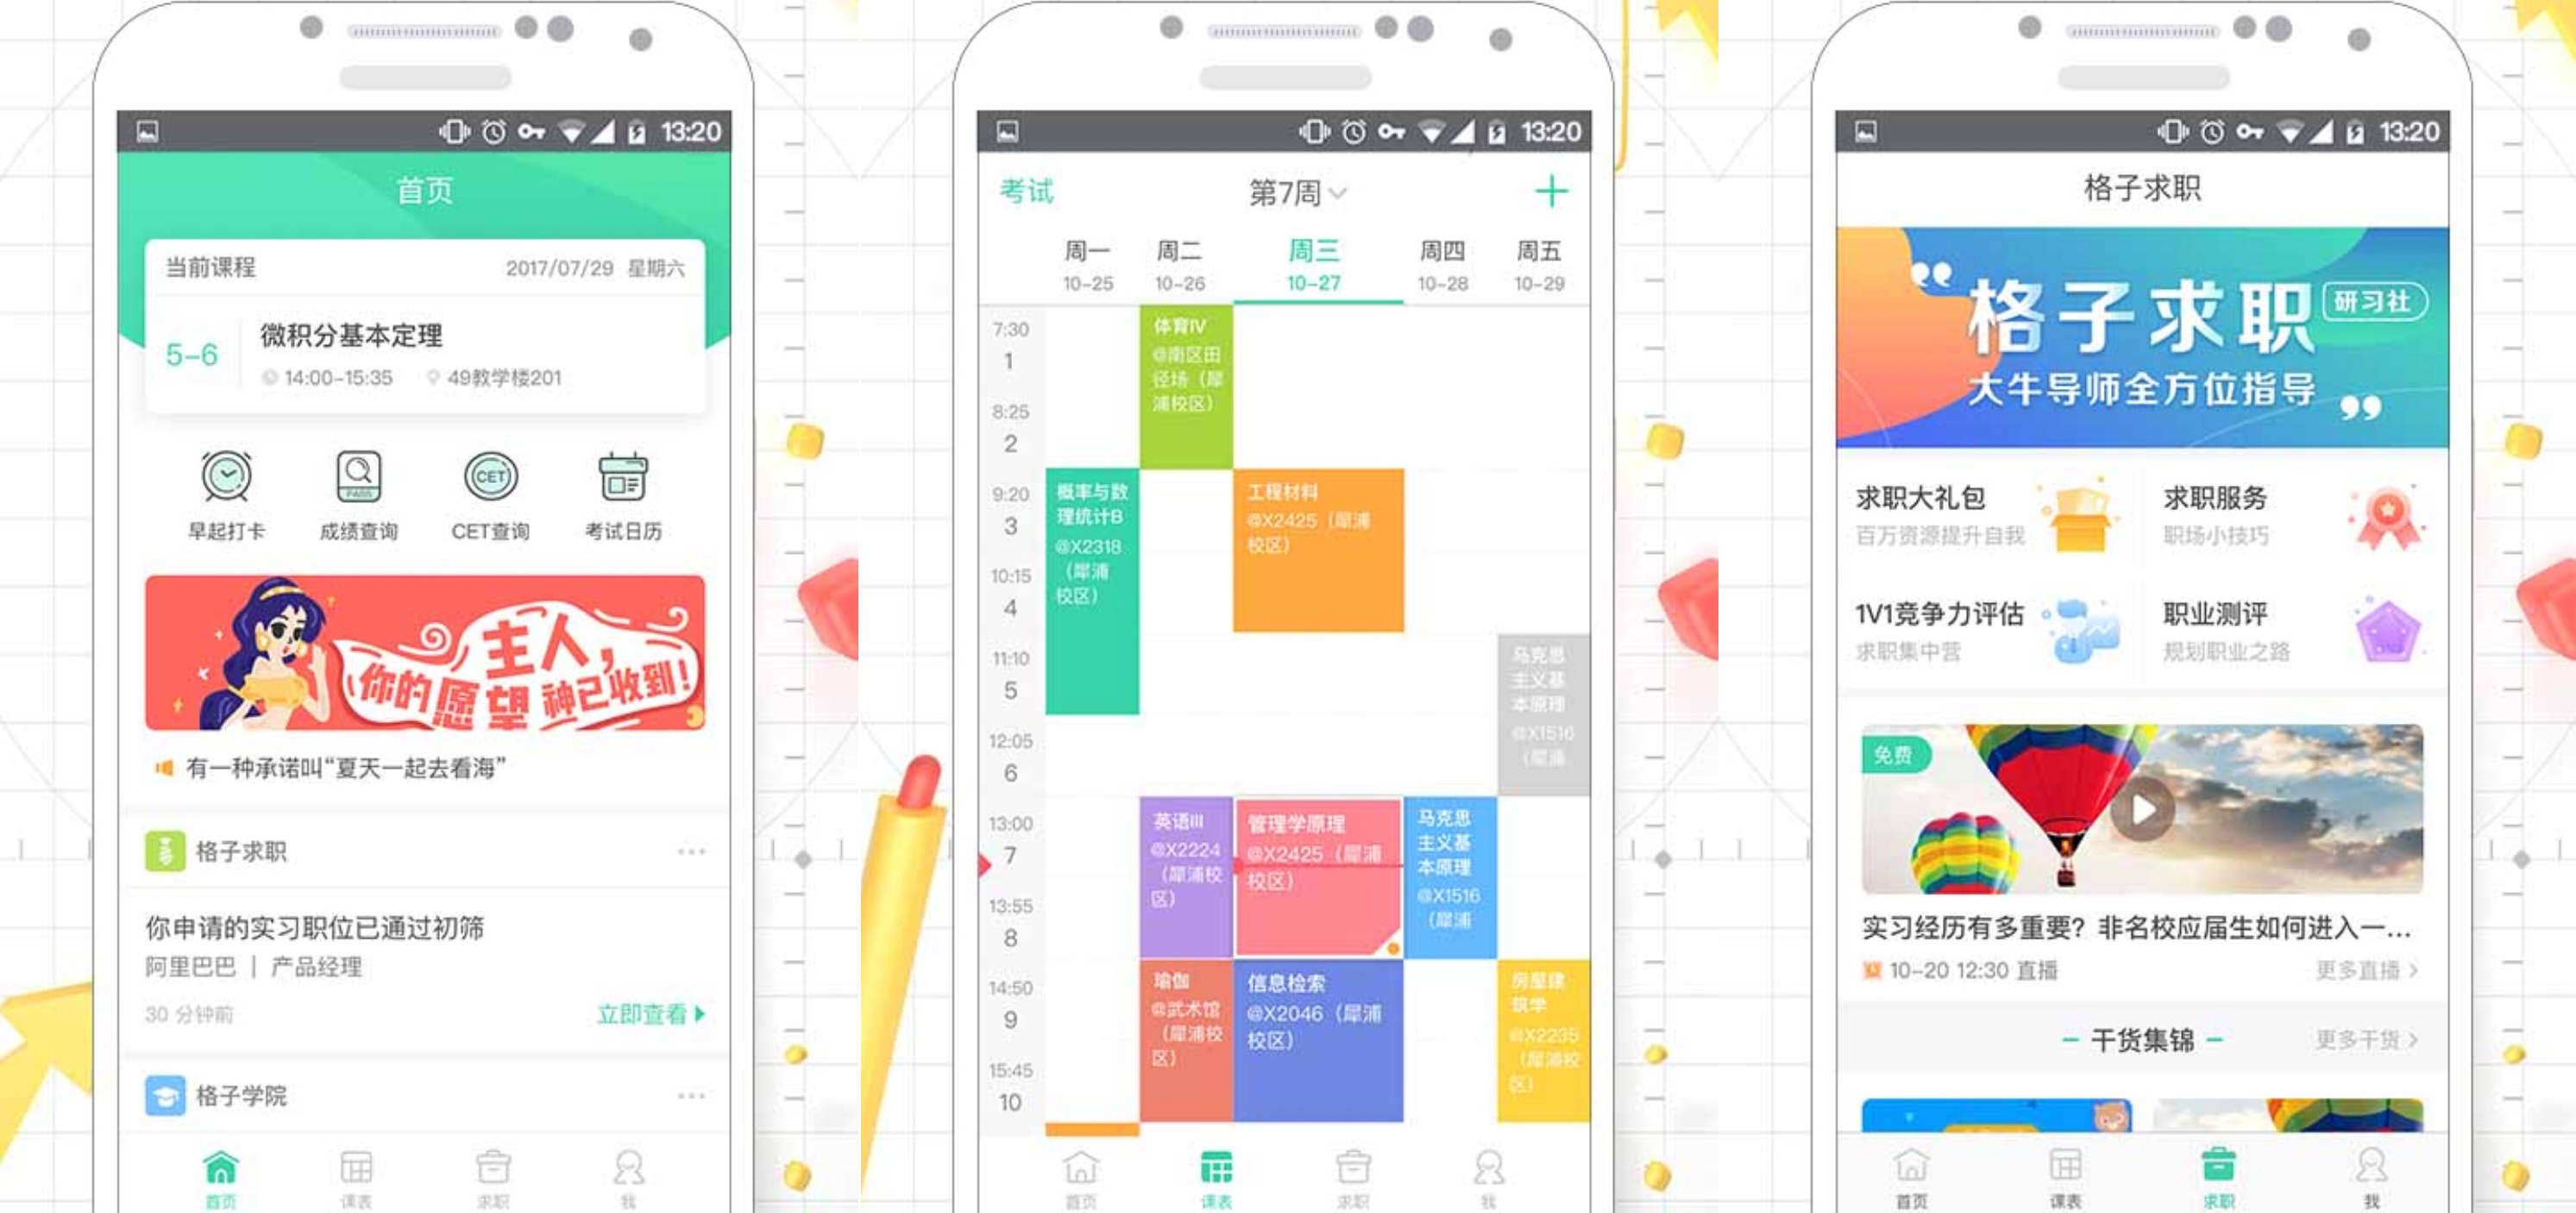
\includegraphics[width=6.5in]{CourseGrid}
    \end{center}
    \begin{enumerate}[i)]

    \item Main Features

    - Quick access to class schedules and 
    docking of more than 1,500 university educational systems.

    - A collection of practical tools, such as CET scores checking.
    
    - Combined with ZAKER News, providing quality reading content.
    
    - Provide a job plaza.

    \item Short-Comings / Possible Improvements
    
    - Too many useless information.

    - Cannot add other schedules or make notes.

    - Cannot provide the GPA review.

    - Cannot access the course schedule of HKU.

    \end{enumerate}


    \subsubsection{SuperCurriculum}
    \begin{center}
        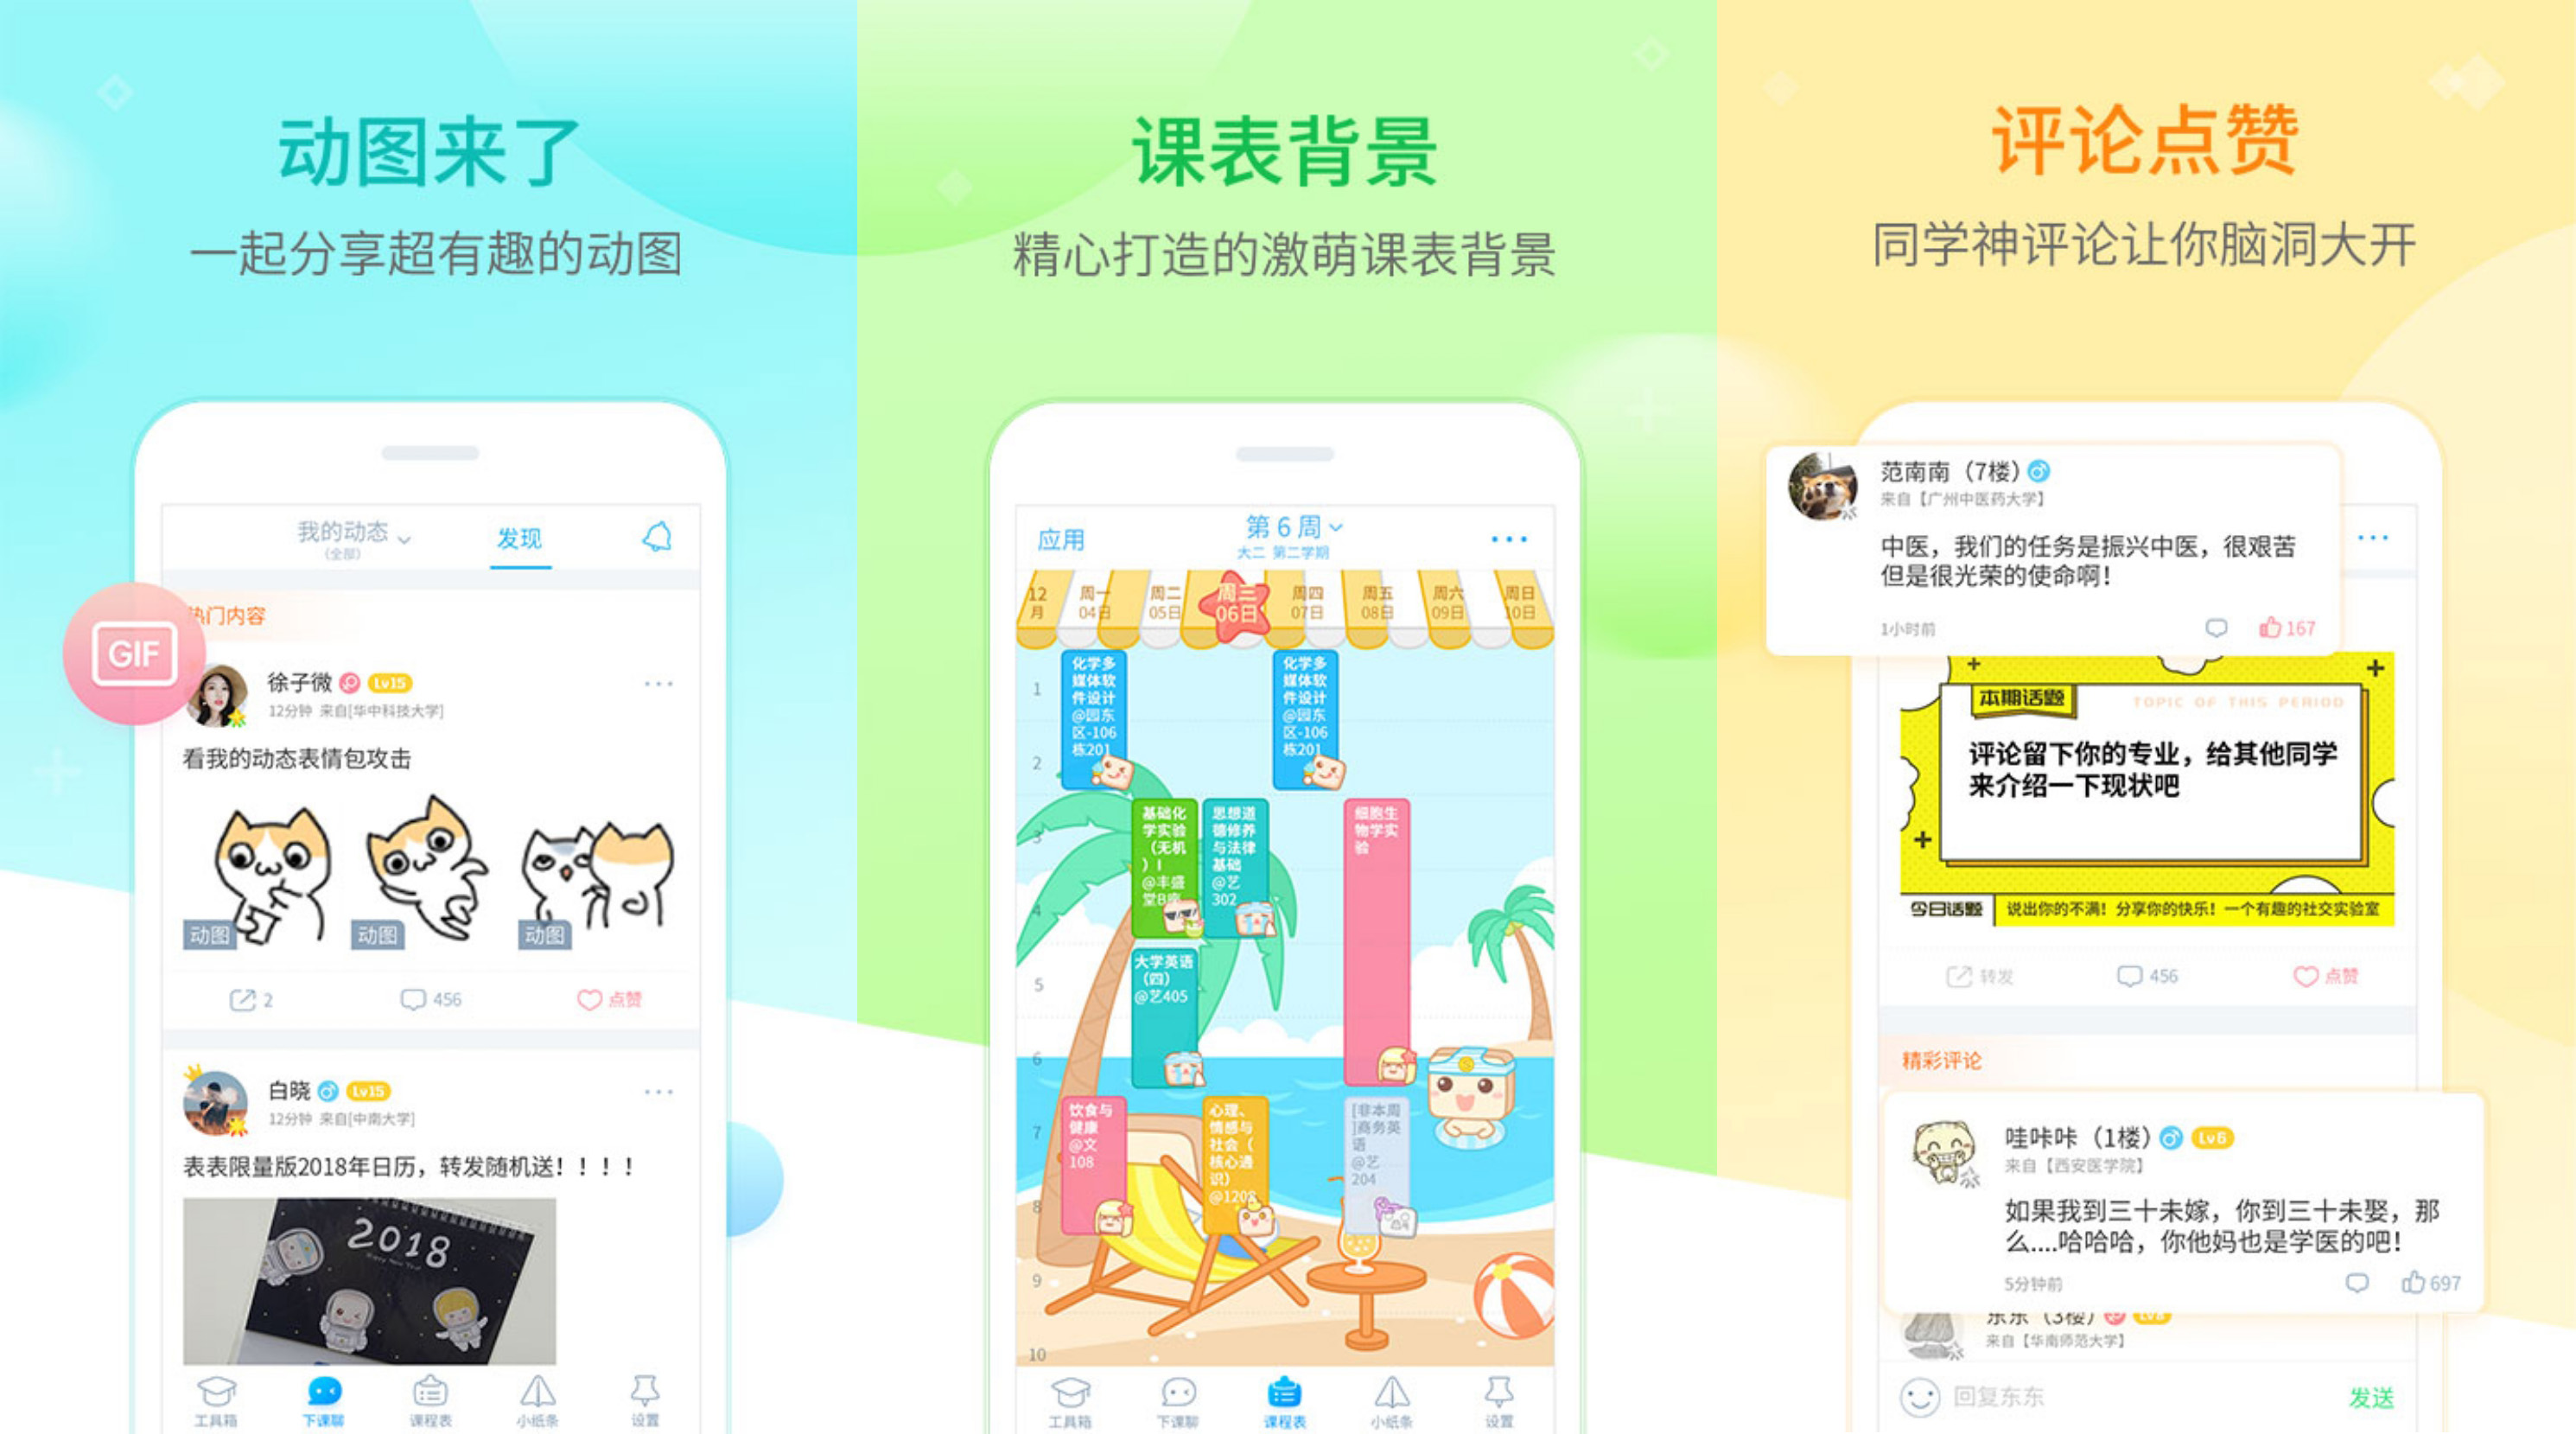
\includegraphics[width=6.5in]{SuperCurriculum}
    \end{center}
    \begin{enumerate}[i)]

    \item Main Features

    - Quick access to class schedules.

    - A collection of practical tools, such as CET scores checking.
    
    - Provide an alumni platform.

    \item Short-Comings / Possible Improvements
    
    - Too many useless information, like a social tool.

    - Cannot add other schedules or make notes.

    - Cannot access the course schedule of HKU.

    \end{enumerate}



    \newpage
    \section{Summary of our Application}

    \subsection{Motivation}
    With the rapid development of mobile networks, 
    it’s very common to bring a smart phone. 
    But when we want to view today’s class schedule or venue, 
    we still need to open HKU page using any browser on the smart phone. 
    The operation is so cumbersome that 
    we want to replace it with a smart, convenient app.
    But in the App store, we could not find a properly App
    to do so, thus we developed this App.

    \subsection{Functions}
    \begin{enumerate}[a)]
    \item Login with HKU Portal UID and PIN
    
    Different student get login in the system with their own HKU
    Portal UID and PIN to view their own courses or use other features. 
    If the UID and PIN is not matched, you will not access other 
    information.

    This also ensures the independence of User data.
    
    \item Personal course schedule
    
    View personal courses here in a time table sort by time, 
    usually in weeks. 

    You can get the whole semester courses information 
    including Holiday and Reading Week information. 
    Whenever you want to see other week's schedule, just click 
    the "Week XX" in the top, and you then can click the week you 
    want to see. Also, you can modify the current week with the 
    information showed in the App.

    Click the course item to get more information about the course,
    such as the instructor and the venue. 
    
    Because data is saved in from remote server, 
    you will not miss any courses.

    \item Add reminder to calendar
    
    You can add a course reminder to calendar 
    by hold the course item. 
    But you still needs to modify the calendar 
    cause this reminder is too simple.
    
    Of course, before doing this,
    you need to permit the app reading/writing your calendar.

    \item Calculate personal GPA
    
    You can use this feature to transform score into 
    GPA by drag the seek bar control.
    This calculator transform the score into GPA by the equation:
    $$GPA =
    \begin{cases}
        max\{1.0, \frac{min\{90, score\} - 50}{10} \} & {score \geq  60}\\
        0 & {score < 60}
    \end{cases}$$

    \item Check personal exam time
    
    You can check out your exam information in blocks, 
    including date, venue, note of each exam.
    The remain days count will give you a precise time 
    to make preparation, 
    and we also listed other things you can bring to the exam,
    such as calculator or A4 paper.

    \item Add/Modify/Delete personal notes
    
    You can manage your notes here. 
    Each note has their own title and body,
    you can only add text here.
    Taking notes at any time may keep you from missing any deadline.
    And modify or delete the notes whenever you want.
    This won't be shared to anyone else.
    \end{enumerate}

    For more information and vivid demonstration, 
    please watch the video.

    \subsection{Framework Design}
    \begin{center}
        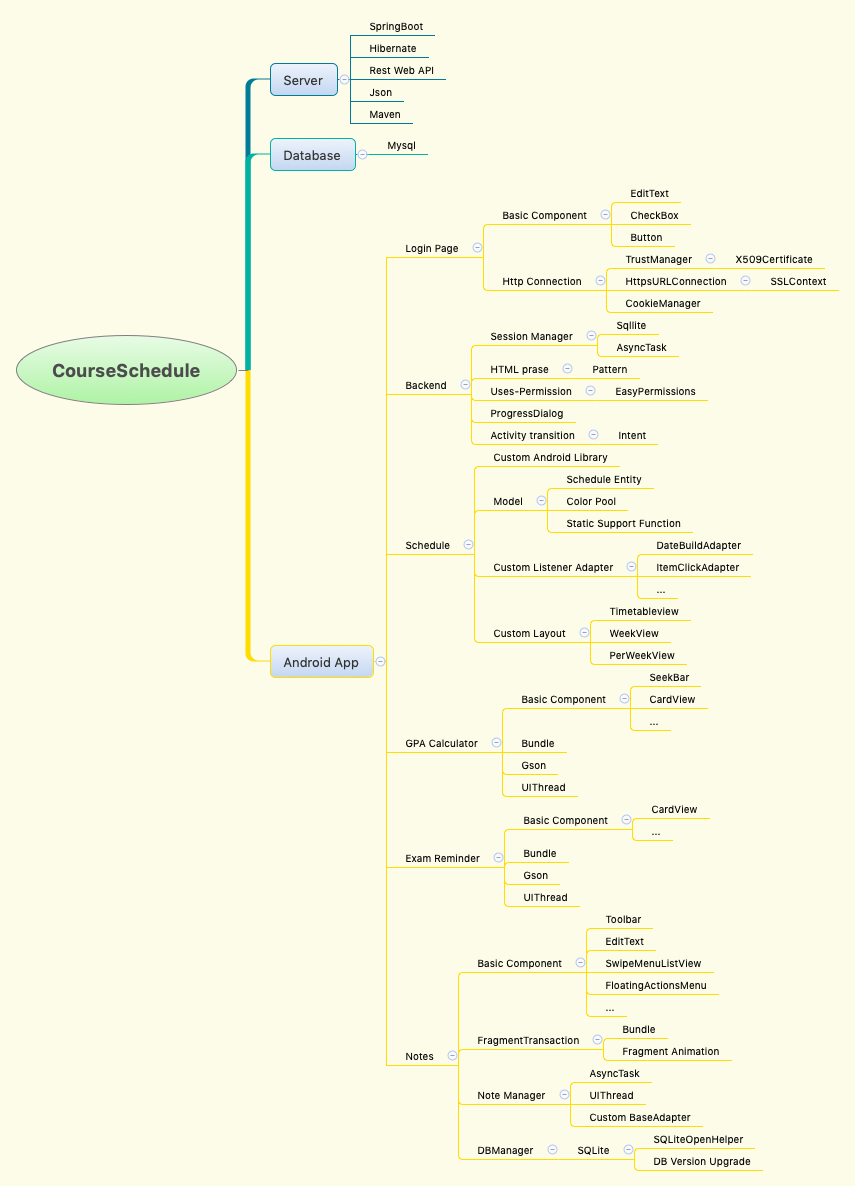
\includegraphics[width=6.3in]{CourseScheduleFramework}
    \end{center}
    
    
 


    
    \section{Contributions}

    \begin{table}[h]
        \centering
        \begin{tabular}{|c|l|}
            \hline
            \multirow{8}{*}{ZHANG Kai} &  Project framework design, feature design\\
            \cline{2-2}
            &The development of Web Server by using spring boot and MySQL \\
            \cline{2-2}
            &Main Activity, corresponding layout xml files \\
            \cline{2-2}
            &Fragment of login page, including corresponding layout xml files \\
            \cline{2-2}
            &Http Connection, including progressing dialog, session manager\\
            \cline{2-2}
            &Uses-permission of Calendar and Internet \\
            \cline{2-2}
            &HTML parse with the use of Gson\\
            \cline{2-2}
            &Complete the draft documentation and Readme.md\\
            \hline
            \multirow{7}{*}{WANG Dezhao} &  
            Provide ideas\\
            \cline{2-2}
            & Custom TimeTableView library. This is an individual library 
            with different views, models, operators and \\
            & listener.\\
            \cline{2-2}
            & Fragment of Schedule, including corresponding 
            layout xml files \\
            \cline{2-2}
            &Fragment of GPACalculator, including corresponding
             layout xml files \\
            \cline{2-2}
            & Fragment of exam reminder, including 
            corresponding layout xml files. \\
            \cline{2-2}
            & Proofread the documentation \\
            \hline
            \multirow{8}{*}{YAN Qiangyu} &  
            Fragment of notes, including corresponding layout xml files.\\
            \cline{2-2}
            & Custom SwipeMenuListView and FloatActionsMenu, 
            with custom basic animation\\
            \cline{2-2}
            & Note Manager with custom BaseAdapter, 
            add/delete/modify personal notes in asynchronous tasks and \\
            & update UI in UIThread. \\
            \cline{2-2}
            & Database Manager, using SQLite to manage the notes information \\
            \cline{2-2}
            & Do background research \\
            \cline{2-2}
            & Make the video \\
            \cline{2-2}
            & Add details and complete the final documentation \\
            \hline
        \end{tabular}
    \end{table}

    \end{document}